\chapter{Evaluation Methods}\label{ch:evaluation-methods}
The last step of the pipeline is to evaluate the results in an automatic way.
We first want to provide a methodology to measure the performance of the \ac{CEP} extraction algorithm.
Second, we want to provide methodologies to evaluate the overall quality of the \ac{WDCG} by using different quality scores.


\section{Performance Measurement Of Cause-Effect Pair Extraction}\label{sec:measure-the-performance-of-the-cause-effect}
In this section, we want to provide a methodology to create a dataset consisting of sentences labeled with multiple \ac{CEP}s.
We then use the performance measurement method from \cite{pawar2021knowledge} as a baseline, which can handle a dataset where each sentence can only have one \ac{CEP}.
We first want to improve the definition of their \qq{matching} criteria by computing the \ac{IoU} between a predicted and labeled \ac{CEP} and deciding based on a threshold value if the pair is \qq{matching}.
We second extend the idea to measure the performance of multiple \ac{CEP}s in the same sentence.

\subsection{Datasets}\label{subsec:datasets}
\begin{figure}
    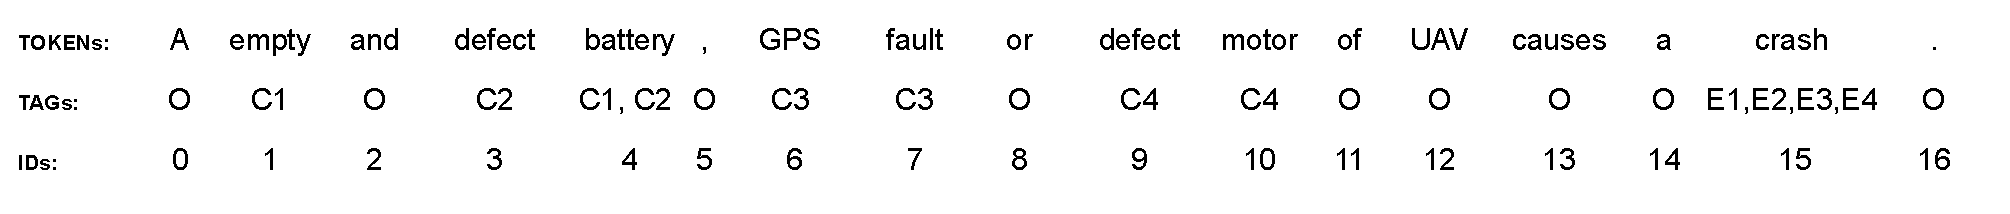
\includegraphics[width=\textwidth]{figures/evaluation_methods/labled_dataset}
    \caption{Labeled Sentence Example}\label{fig:labeled-sentence}
\end{figure}
In this subsection, we want to describe two benchmark datasets that can be used to measure the performance of a \ac{CEP} extracting algorithm.
We followed the \qq{event sequence block label} method from \cite{xu2020review} to create our benchmark datasets.
In \autoref{fig:labeled-sentence} we can see how such labeling look on the sentence \qq{A empty and defect battery, GPS fault or defect motor of UAV causes a crash}.
This labeling technique splits a sentence into tokens and then assign to each token a specific label which can be either \qq{C} cause, \qq{E} effect, or \qq{O} other.
Moreover, to solve the multiple causality problem, we can assign to the \qq{C} and \qq{E} tag an ID such as \qq{C1} or \qq{E1}, to divide different \ac{CEP}s.

\subsubsection{Nato-SFA Dataset}\label{subsubsec:nato-sfa}
In \cite{Hassanzadeh19}, the authors provided the \ac{NATO-SFA} benchmark dataset, which \qq{examines the main trends of global change and the resultant defense and security implications for NATO}\footnote{\url{https://www.act.nato.int/images/stories/media/doclibrary/171004_sfa_2017_report_hr.pdf}}.
Their dataset contains 118 pairs where the first 59 are \ac{CEP} and the other 59 pairs have no causal relations.
Unfortunately, the authors only provided the extracted pairs and the methodology for extracting these pairs.
Thus their dataset does not provide the source sentences of the pairs.
Furthermore, the authors only handle single \ac{CEP}s.
Therefore, we followed their methodology to create a dataset based on their extractions and the report.
We were able to find 100 sentences that are represented in their dataset.
We then used the tokenizer from spaCy to split the sentence into multiple tokens.
Next, we labeled each token manually based on the pairs from the original dataset.
Furthermore, some of the \ac{CEP}s include conjunction, which we manually divided into independent \ac{CEP}s.
We want to use this dataset to compare our results with a dataset from a different domain with high-quality sentences and less noise.

\subsubsection{ArduPilot Dataset}\label{subsubsec:ardupilot}
To measure the performance of the \ac{CEP} extraction, particular for our domain, we created a dataset based on the sentence we gathered during scraping.
This dataset currently contains 69 sentences, where 20 did not include causation, 32 included a single \ac{CEP} and 17 multiple \ac{CEP}s.
Furthermore, we also included some linguistic features in the dataset.
These could potentially be useful if we want to extend the \ac{CEP} algorithm with a machine learning solution, which uses the linguistic tags as features during training.
In the dataset, we have the following columns:
\begin{itemize}
    \item id - integer: This id represents the unique id from the sentence from which we extracted the token.
    \item token - string: Represents the raw text information of the token.
    \item tag - string: This defines the label of the token (see. \autoref{fig:labeled-sentence})
    \item token\_id - integer: The id of the token in the sentence represents the order of the tokens (see \autoref{fig:labeled-sentence}).
    \item lemma  - string: The lemmatized representation of the token.
    \item pos  - string: The \ac{POS} tag for the token.
    \item dep  - string: The \ac{DEP} tag for the token.
\end{itemize}

\subsection{Performance Measurement}\label{subsec:performance-measurement}
\begin{figure}
    \begin{center}
        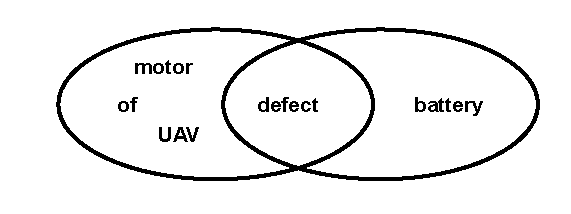
\includegraphics[scale=.85]{figures/evaluation_methods/jaccard_similarity}
        \caption{Jaccard Similarity}\label{fig:jaccard-similarity}
    \end{center}
\end{figure}
In \cite{pawar2021knowledge} the authors defined a match between two \ac{CEP}s when at least one word between the cause phrases is matching as well as between the effect phrases.
Thus, \qq{defect motor of UAV} => \qq{crash} and \qq{defect battery} => \qq{crash} would be matching because \qq{defect} and \qq{crash} are in both phrases.
Instead of using a fixed rule, we want to calculate the \ac{IoU} between two \ac{CEP}s and compare the \ac{IoU} with a threshold value to decide if the \ac{CEP}s are \qq{matching}.
To calculate the \ac{IoU}  between two \ac{CEP}s, we first calculate the \ac{IoU}  between the cause phrases and, accordingly, the effect phrases.
Fortunate, the Jaccard similarity defines the \ac{IoU} between two phrases:
\begin{equation}
    \label{eq:jaccard-similarity}
    J(P1, P2) = \frac{\left| P1 \cap P2 \right|}{\left| P1 \cup P2 \right|}
\end{equation}
In \autoref{fig:jaccard-similarity} we see a graphical representation of the Jaccard similarity between the two phrases \qq{defect motor of UAV} and \qq{defect battery}.
In this example, the Jaccard similarity is $1/5$, thus 0.2. However, the Jaccard similarity between the textual representations of phrases could lead to unintentional errors because we cannot differentiate between textual tokens.
Thus, in our previous example, the \ac{IoU} should be 0 because the \qq{defect} of both phrases represents a different token in the sentence (see \autoref{fig:labeled-sentence}).
To have distinct representations of the tokens, we use the \qq{token\_id} of the labeled dataset and the predictions.
We defined the \ac{IoU} between two \ac{CEP}s by calculating the harmonic mean between the \ac{IoU}  of the cause phrases and the \ac{IoU} of the effect phrases with:
\begin{equation}
    \label{eq:iuo-cause-effect-pair}
    IoU\_CEP(cause\_IoU, effect\_IoU) = 2*\frac{cause\_IoU*effect\_IoU}{cause\_IoU+effect\_IoU}
\end{equation}
After calculating \ac{IoU} between two pairs, we can define the \qq{matching} term by comparing the \ac{IoU}  with a threshold:
\begin{equation}
    \label{eq:matching}
    Matching(IoU, threshold) = \left\{
    \begin{array}{ll}
        True  & IoU > threshold  \\
        False & IoU <= threshold \\
    \end{array}
    \right.
\end{equation}
A \ac{TP} is counted for each labeled pair in the dataset if there is a \qq{matching} predicted pair and a \ac{FN} otherwise.
Also, a \ac{FP} is counted for each predicted pair if there is no \qq{matching} labeled pair in the dataset.
Precision, Recall, and F1-score are computed as follows:
\begin{equation}
    \label{eq:measurement-scores}
    Precision = \frac{TP}{TP+FP}
    \quad\mathrm{,}\quad
    Recall = \frac{TP}{TP+FN}
    \quad\mathrm{,}\quad
    F1 = 2*\frac{Precision*Recall}{Precision+Recall}
\end{equation}
We can now calculate the performance measurement scores on different threshold values, which allows us to create a 2d-plot with threshold values ranging from 0 to 1 on the x-axis and performance scores on the y-axis (see \autoref{ch:results}).


\section{Find Cause-Effect Pairs In The Flight Logs}\label{sec:find-cause-effect-pairs-in-the-uav-logs}
This section provides different quality scores to evaluate the \ac{WDCG}.

\subsection{Graph Matching}\label{subsec:graph-matching}
We want to lay the foundation of the following quality scores in this subsection.
We can perform two types of queries on a \ac{WDCG}.
The first query takes a node as input and responds with the amount of \qq{matching} nodes in the graph.
We can calculate the amount by summing all weights from the edges connected with the search node.
Thus, if we have as input \qq{empty battery}, we would get a total of 12 mentions (see \autoref{fig:causal-graph}).
The second query represents an edge consisting of two nodes, where the response is the weight of all \qq{matching} edges in the graph.
Thus, if we have as input \qq{empty battery} =>\qq{crash} we get a total of 3 mentions returned.
The previous examples represent exact matching between the nodes or edges.
However, if we have an input like \qq{battery} => \qq{crash} the graph did not have the exact representation of the pair.
We want to use the same idea from the previous section to use \ac{IoU} with a threshold value to decide if such a query is \qq{matching}.

\subsection{Diversity Of A Graph}\label{subsec:diversity-of-graph}
We define the diversity of a node by the fraction between the number of explicit mentions and the number of mentions when making a query based on a threshold value.
For example, the node \qq{empty battery} would lead to 12 explicit mentions and 17 mentions with a threshold value of 0.6 because we also count the mentions for \qq{defect battery}.
The diversity can be defined as follows:
\begin{equation}
    \label{eq:node-diversity}
    node\_diversity(thresh) = \frac{exact\_node\_mentions}{node\_mentions(thresh)}
\end{equation}
\begin{equation}
    \label{eq:edge-diversity}
    edge\_diversity(thresh) = \frac{exact\_edge\_mentions}{edge\_mentions(thresh)}
\end{equation}
Thus for the node \qq{empty battery} we would have a diversity of $12/17=0.706$ at threshold 0.6.
The diversity ranges from 0.0 to 1.0, where 1.0 indicates that no other representation for this information is in the \ac{WDCG}.
A low diversity score indicates multiple nodes with similar meanings.
Thus, the same information in the graph is spread to different nodes.
To calculate the diversity for the whole graph, we calculate the diversity for each node and take its mean.
We can calculate the diversity for different threshold values in a similar to \autoref{subsec:performance-measurement}.
We calculate the diversity for a node and an edge similarly.

\subsection{Consistency Of The Edges}\label{subsec:consistency-of-the-edges}
The consistency score defines the quality of an edge by comparing it with the direct contradiction.
In general if there is a causality like \qq{empty battery} => \qq{crash"} \qq{crash} => \qq{emtpy battery} would be the direct contradiction.
We calculate consistency by first calculating the number of mentions of the edges ($edge\_mentions$)and the number of mentions where we swap the direction of the relation of the edge ($reversed\_edge\_mentions$):
\begin{equation}
    \label{eq:consistency-score}
    consistency(thresh) = \frac{edge\_mentions(thresh)}{edge\_mentions(thresh) + reversed\_edge\_mentions(thresh)}
\end{equation}
Thus if 10 users would say \qq{empty battery} => \qq{crash} and only one user \qq{crash} => \qq{emtpy battery} we would have a consistency score for the first edge of ~''0.91'', whereas for the second edge ~''0.09''.
The consistency score ranges between 0.0 and 1.0, where 1.0 means no contradictions.
A consistency score of 0.5 can be interpreted that the users are not sure about the relation of the nodes.
On the other hand, a score near 0.0 indicates that the majority disagree with this edge.


\subsection{Information Score}\label{subsec:information-score}
We want to provide a measure representing the information value of an edge.
Therefore, we define the information of an edge with:
\begin{equation}
    \label{eq:information-score}
    information(thresh) = consistency(thresh) * edge\_mentions(thresh)
\end{equation}
For example the edge \qq{empty battery} => \qq{crash} would have a information score of $0.91 * 10=9.1$.
This score reflects how often an edge is mentioned and penalties edges that have contradictions.
Based on the information score, we define an edge as valuable with:
\begin{equation}
    \label{eq:value_edge}
    valuable(information) = \left\{
    \begin{array}{ll}
        True  & information > 1  \\
        False & information <= 1 \\
    \end{array}
    \right.
\end{equation}
Thus, an edge can only be valuable when mentioned at least two times.
Furthermore, an edge cannot be valuable when the edge has too many contradictions.

\subsection{Coverage Between Two Graphs}\label{subsec:coverage-between-two-graphs}
The coverage score represents how many nodes/edges are reflected in a target graph.
To calculate the score, we assign a boolean label to each node/edge in the source graph that indicates if the node/edge is reflected in the target graph.
The coverage score for the graph is the fraction between the number of true labels and the number of the total nodes/edges.
Thus, if we have a source graph of 1000 nodes and a target graph of 50 nodes where 25 nodes match both, we would have coverage of \qq{2,5\%} for the source graph and \qq{50\%} for the target graph.

\subsection{Correctness Of Graph}\label{subsec:correctness-of-graph}
The correctness of the causal graph can be measured by considering the flight log graph as the ground truth.
We assign a correct label to each edge, which can be \qq{correct}, \qq{incorrect}, or \qq{unknown} based on the valuable label.
We use the edge from the source graph as the input for the matching query on the target graph to find if the edge is also detected as valuable in the target graph.
We define the edge as \qq{unknown} if the \qq{information} of the target graph is 0 because there is no evidence in the target graph, which means that we cannot deduct the correctness of the edge.
However, if there is evidence in the target graph, we define the edge as correct if the edge is valuable in the source graph and the target graph; otherwise, we define it \qq{incorrect}.
To calculate the correctness of the whole causal graph, we use:
\begin{equation}
    \label{eq:correctness}
    correctness(thresh) = \frac{correct\_edges(thresh)}{correct\_edges(thresh) + incorrect\_edges(thresh)}
\end{equation}
